\documentclass[12pt]{article}

\usepackage{fancyhdr} %for headers
\usepackage[margin=1.0in]{geometry} % margin size (can change units)
\usepackage{setspace} % setting spaces in title

\usepackage{cite} % for references

\usepackage{graphicx}

\usepackage{floatrow} % to add side by side tables with figures

\usepackage{booktabs} % adding in table support

\usepackage{amssymb} % more symbols

\usepackage{subcaption}

\renewcommand{\arraystretch}{1.3} % make tables a bit larger (vertically)
\setlength{\tabcolsep}{10pt}	  % make the table width larger
\newdimen\heavyrulewidth
\newdimen\lightrulewidth
\heavyrulewidth=.12em  %make the top rule of a table heavy
\lightrulewidth=.05em  %and the line below the titles a bit lighter

\usepackage{multirow}

%% Nice lists
\usepackage{scrextend}
\addtokomafont{labelinglabel}{\sffamily}

\usepackage{etoolbox}   % for booleans and much more
\usepackage{verbatim}   % for the comment environment

\pagenumbering{arabic}

% Table float box with bottom caption, box width adjusted to content
\newfloatcommand{capbtabbox}{table}[][\FBwidth]

\usepackage[pdftex]{hyperref} %to add hyperlinks to the referenced pages for easier navigation

\hypersetup{
	colorlinks,
	allcolors=black
}

\newcommand{\e}[1]{\times10^{#1}}

\headheight = 18pt

\widowpenalties 1 10000
\raggedbottom

%% Here is bool logic to turn on or off the sections we wish to have


% setup a new booleans
\newbool{fullreport_bool}
\newbool{prelab_bool}
\newbool{data_bool}
\newcommand{\ExperimentTitle}{}
\newcommand{\ExperimentSubtitle}{Experiment \#}
\newcommand{\HeaderExperimentTitle}{}

\newcommand{\CourseCode}{ECE 331}
\newcommand{\CourseName}{Electronic Devices}
\newcommand{\CourseSection}{Section 203}

\newcommand{\AuthorOneFirstName}{William}
\newcommand{\AuthorOneLastName}{Ngana}
\newcommand{\AuthorOneStudentNumber}{20533462}

\newcommand{\AuthorTwoFirstName}{Michael}
\newcommand{\AuthorTwoLastName}{Hamel}
\newcommand{\AuthorTwoStudentNumber}{20519421}

\newcommand{\UniversityName}{University of Waterloo}
\newcommand{\UniversityLocation}{Waterloo, ON}

\newcommand{\DatePerformed}{February 28, 2018}
\newcommand{\DateSubmitted}{March 9, 2018}

\pagestyle{fancy}
\fancyhf{}
\rhead{\AuthorOneLastName, \AuthorTwoLastName}
\lhead{\CourseCode}
\chead{\HeaderExperimentTitle}
\cfoot{Page \thepage}
\newpage

%% This is a bit messy, but it allows you to hide the different configurations of the document as we need for each submission. This allows you to set a section as hidden, true means hidden.

\setbool{fullreport_bool}{false}
\setbool{prelab_bool}{true}
\setbool{data_bool}{true}

% new environments
\newenvironment{fullreport}{}{}
\newenvironment{prelab}{}{}
\newenvironment{data}{}{}

% set conditional behaviour of environment
\ifbool{fullreport_bool}{\AtBeginEnvironment{fullreport}{\comment}
\AtEndEnvironment{fullreport}{\endcomment}}{}

\ifbool{prelab_bool}{\AtBeginEnvironment{prelab}{\comment}%
\AtEndEnvironment{prelab}{\endcomment}}{}

\ifbool{data_bool}{\AtBeginEnvironment{data}{\comment}%
\AtEndEnvironment{data}{\endcomment}}{}
\begin{document}

% % % %  Full Report   % % % %

\begin{fullreport}
    \thispagestyle{empty}

\newcommand{\HRule}{\rule{\linewidth}{0.5mm}}

\begin{center}

\textsc{\LARGE \UniversityName}\\[1cm]
\textsc{\Large \CourseName}\\[.25cm]
\textsc{\Large \CourseCode}\\[3cm]

\HRule \\[0.7cm]
{ \Huge \ExperimentTitle \\ \vspace{0.4cm}
\Large \textsc{\ExperimentSubtitle}}\\[0.4cm]
\HRule \\[3cm]


% % ---- Two authors style
\Large \emph{Authors:}\\
\AuthorOneFirstName \textsc{ \AuthorOneLastName}\\
\AuthorOneStudentNumber\\[0.4cm]


\AuthorTwoFirstName \textsc{ \AuthorTwoLastName}\\
\AuthorTwoStudentNumber\\[1cm]

\vfill

\UniversityLocation\\

\vspace{5mm}

Date Performed: \DatePerformed\\
Date Submitted: \DateSubmitted

\end{center}
    \section{Prelab}
    \begin{enumerate}
\item[1.]
\begin{figure}[ht]
    \centering
    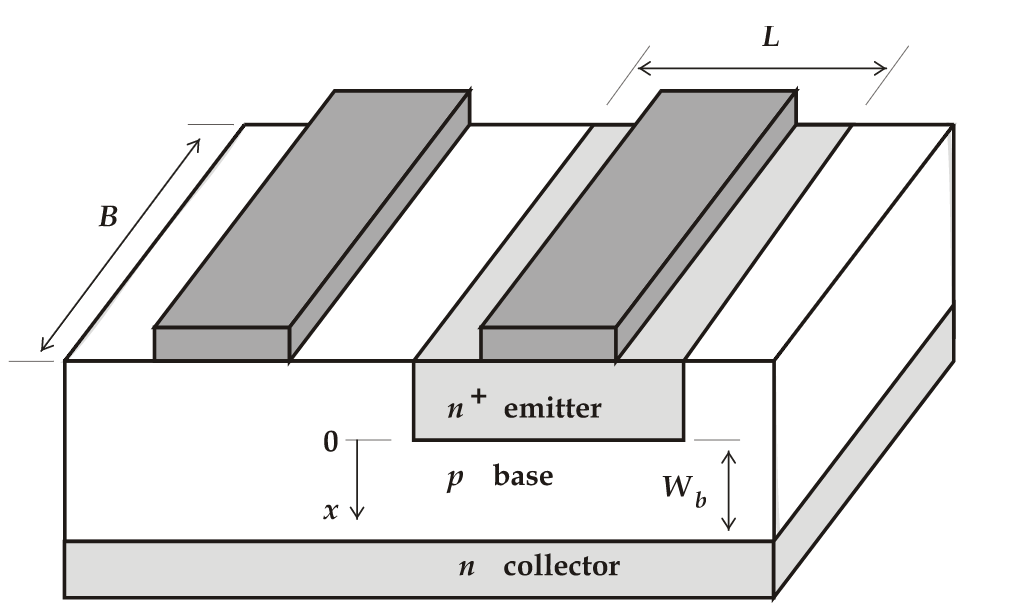
\includegraphics[width=\linewidth]{figures/simple_transistor.PNG}
    \caption{Figure 4 from the lab manual of a simple transistor}
    \label{fig:transitor}
\end{figure}
The figure above is that of a simple transistor from the lab manual. The formula for $I_{CS}$ is:
\begin{equation}
    I_{CS} = \frac{q A_e n_i^2 D_n}{N_{Ab}W_b}
\end{equation}
so if you increase $W_b$ then you are going to lower the gain $\beta_F = \frac{I_C}{I_B}$, but it will increase the switching time


\item[2.]
The three types of materials are:
\begin{labeling}[:]{N\texttt{+} type}
\item [N\texttt{+} type] a n-type semiconductor with a high, often degenerate doping concentration.
\item [N type] a semiconductor that having more conduction electrons than mobile holes.
\item [P type]  a semiconductor having a density of mobile holes in excess of that of conduction electrons.
\end{labeling}


\item[3.]
The four transistor operation modes are:
\begin{labeling}{Reverse-Active}
\item [Saturation] The transistor acts like a short circuit. Current freely flows from collector to emitter.
\item [Cut-off] The transistor acts like an open circuit. No current flows from collector to emitter.
\item [Active] The current from collector to emitter is proportional to the current flowing into the base.
\item [Reverse-Active] Like active mode, the current is proportional to the base current, but it flows in reverse. Current flows from emitter to collector (not, exactly, the purpose transistors were designed for).
\end{labeling}

\item[5.]
The current gain $\beta$ is theoretically constant, but as the question states at high and low values of $I_C$ we see that the the gain decreases. This is due to leakage mechanism in the transistor for low $I_C$ and  due to high level injection for high $I_C$.
\item[6.]
\begin{labeling}{Gummel Plot}
\item [Gummel Plot] A plot which shows $I_C$ versus $V_{BE}$ characteristics of a transistor, this is completed on a semi-log plot where the current is on the log scale.
\item [I\textsubscript{CS}] The collector saturation current is where the base current so that the emitter-base junction is forward biased. In fact, the base current has increased beyond the point where it can cause the collector current flow to increase. At this point, collector emittor currents have increased to a maximal value.
\item [D\textsubscript{n av}] D\textsubscript{n} is the electron diffusion coefficient in the base, which is a physical constant which describing how electrons move through the p-type base. The D\textsubscript{n av} is simply the average of this value throughout the material.
\end{labeling}

\item[7.] The reason that the current gain $\beta \left( \frac{I_C}{I_B} \right) $ decreases at low values of $I_C$ is clear, the ideal model of gain which is shown by $\beta  = \frac{I_C}{I_B}$ is accurate, and hence  $I_C \propto \beta$.

However the reason that the current gain decreases at high values of $I_C$ is not as simple, we deviate from the ideal line equation due to the base resistance and emitter  resistance of the transistor. These resistances are only relevant at high currents as they are non-idealities.

%This is caused because the Voltage ($V_{BE}$) is maintained at a constant value, but when the currents through the device become large the resistances of the emittor and base become significant. This is modelled through the equation: $V_{BE eff} = V_{BE} - \frac{I_{C}}{\beta} r_{bb} - \frac{I_{C}(\beta - 1)}{\beta} r_e$ where $r_e$ and $r_{bb}$ are the emittor and base resistance respectively. There are also other high current effects that come into play


\item[8.]
The differences between the different types of resistors are:
\begin{labeling}{P type pinched resistor}
\item [P type pinched resistor] is a n type region surrounded by a thin p region, known as the pinching region, which is again covered by a n region. It works by lowering the crossectional area and only allowing a small reverse current. These types of resistors can have very high resistances but are often more difficult to manufacture.
\item [P type resistor] is a formed in any one of the isolated regions of p doping, surrounded by a n-region. The differences in resistance are generally controlled by the doping and then crossectional area can also be controlled, but is much larger than the pinched resistors as we only have two layers. 
\item [Carbon resistor] is not a solid state resistor and is not created by using deposition. These different resistance values are generated by varying the length of resistive material that the electricity passes through. This resistive material is made of graphite, ceramic dust and resin.
\end{labeling}

\item[9.]

We see here that the figure below has both the pinched and non-pinched p-type resistor. We know that the calculation of the cross-sectional area will be height times thickness of the resistive material. We note that in our figures, the height will be consistant between both the pinched and unpinched resistor, however the thickness will not be. The thickness of the p-type material will be $t_p$, but the thickness of the pinched resistor will be $t_p - t_n$, since it is deposited above it. This difference in thicness will decrease the area, and effectively increase the resistance.


\begin{figure}[h]
    \begin{subfigure}[b]{\linewidth}
    \centering
    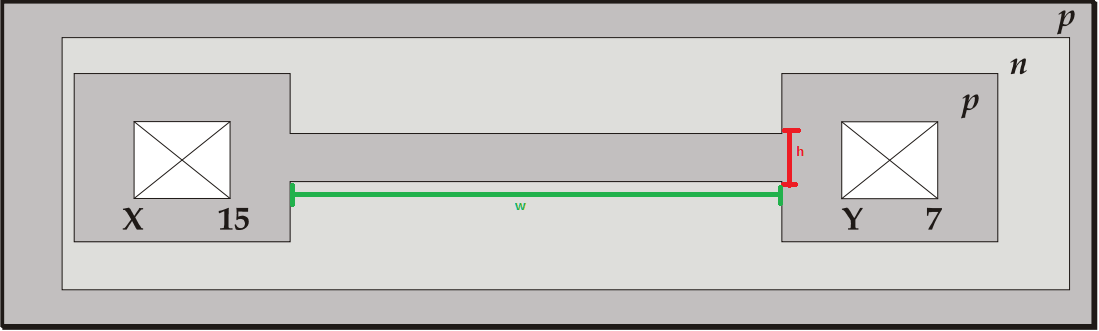
\includegraphics[width=0.95\linewidth]{figures/p_resist.png}
    \caption{Top down diagram of a p-type resistor}
    \label{fig:p_resist}
    \end{subfigure}
    \begin{subfigure}[b]{\linewidth}
    \centering
    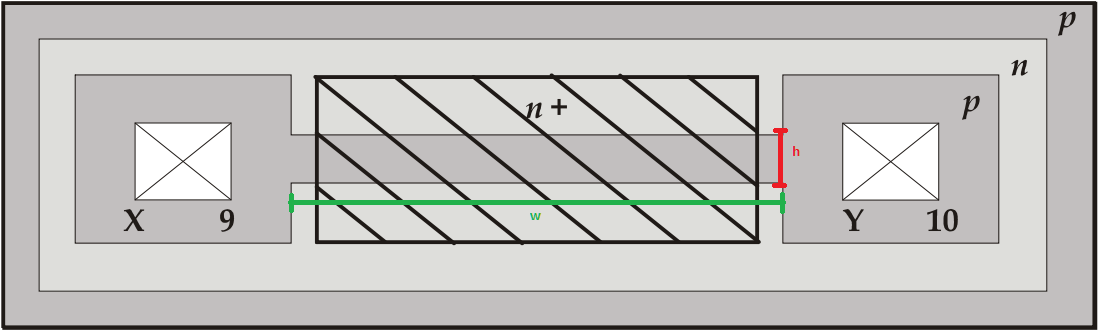
\includegraphics[width=0.95\linewidth]{figures/p_pinched_resist.png}
    \caption{Top down diagram of a p-type pinched resistor}
    \label{fig:pinched_resist}
    \end{subfigure}
\end{figure}

\end{enumerate}

    \clearpage
    \section{In-Lab Data Collection}
    \subsection{Standard Downward Characteristics}
$R_B = 10.16 \Omega$\\
$R_C = 287.7 \Omega$\\
Here we will study $I_C$ vs $V_{BE}$ characteristics and $\beta$ versus $I_C$ characteristics.

\begin{table}[ht]
    \begin{tabular}{cccc}
\hline
\textbf{$V_{BE}$ (mV)} & \textbf{$I_{B}$ } & \textbf{$V_{CE}$ (V)} & \textbf{$I_{C}$ } \\ \hline
\textit{\textbf{500}} & 0.027 $\mu A$& 1.500  & 0.14 $\mu A$ \\
\textit{\textbf{550}} & 0.088 $\mu A$& 1.500  &0.92  $\mu A$ \\
\textit{\textbf{600}} & 0.280 $\mu A$& 1.499  & 6.02  $\mu A$ \\
\textit{\textbf{650}} & 0.956 $\mu A$&1.500  & 39.76 $\mu A$ \\
\textit{\textbf{700}} & 3.541 $\mu A$ & 1.500  & 259.0 $\mu A$\\
\textit{\textbf{750}} & 0.01295 mA & 1.503  & 1.3666 mA\\
\textit{\textbf{800}} & 0.03919 mA & 1.503  & 4.6170 mA\\
\textit{\textbf{850}} & 0.09654 mA  & 1.523  & 9.1807  mA\\\hline
\end{tabular}
    \caption{Standard Downward Characteristics for transistor 1}
    \label{tab:down}
\end{table}


\subsection{Upwards Operation}

Here we look at the upwards gain of transistor 1 as a function of voltage.

\begin{table}[ht]
    \begin{tabular}{ccccc}
\hline
\textbf{$V_{BE}$ (mV)} & \textbf{$I_{B}$} & \textbf{$V_{CE}$ (V)} & \textbf{$I_{C}$} & $\beta$\\ \hline
\textit{\textbf{550}} & 0.237 $\mu A$ & 1.500  & 1.24  $\mu A$ & 5.232 \\
\textit{\textbf{600}} & 1.465 $\mu A$ & 1.500  & 7.82  $\mu A$ & 5.337 \\
\textit{\textbf{650}} & 9.675 $\mu A$ & 1.501 & 54.82 $\mu A$ & 5.666 \\
\textit{\textbf{700}} & 44.564 $\mu A$ &1.504  & 274.16  $\mu A$ & 6.152\\
\textit{\textbf{750}} & 0.17097 mA & 1.507  & 1.0551 mA  & 6.171\\
\textit{\textbf{800}} & 0.52758 mA & 1.500  & 2.7671 mA & 5.244\\\hline
\end{tabular}
    \caption{Standard Upwards Characteristics for transistor 1}
    \label{tab:up}
\end{table}


\subsection{Base Resistance}

Total Resistance between X and Y in pattern 1 is: $5.021 k \Omega$

Total Resistance between X and Y in pattern 2 is: $61.7 k \Omega$


\subsection{Lateral \textit{pnp} Devices}


We can measure the gain of the lateral pnp transistor by taking the current values of $I_B$ = 0.1007 mA \& $I_C$ = 1.0460 mA at values of $V_CE$ = -1.50 V. This gives a gain of 10.4526. \\

 %\& $V_BE$ = -0.655

We can also measure the gain of the lateral pnp transistor where the outer p diffusion is used as an emitter and the center p diffusion is used as the collector. The value of gain that we get with the currents of $I_B$ = 0.1000 mA\& $I_C$ = 0.0404 mA at values of $V_CE$ = -1.50 V. Giving us a gain of 0.404.

%\& $V_BE$ = -0.691

    \clearpage
    \section{Post Lab Data Analysis}
    \subsection{MOSFET Threshold Voltage}
 The first part of this analysis was to determine the values of $I_{DS}$ and $\sqrt{I{DS}}$ and put them into a table which is below.
 
 \begin{table}[h]
    \begin{tabular}{@{}cccccc@{}}
\toprule
\textbf{$V_{BB}$ (V)} & \multicolumn{1}{l}{\textbf{$V_{GG}$ (V)}} & \textbf{$V_{DD}$ (V)} & \textbf{$V_{DS}$ (V)} & \textbf{$I_{DS}$} & \textbf{$\sqrt{I_{DS}}$} \\ \midrule
%                        VGG     VDD     VDS     IDS  sqrt(IDS)
\textit{\textbf{0}}     &  2.86     &   7.09    &  6.0550     & 1.0108    & 1.0054 \\
\textit{\textbf{0}}     &  3.60     &   8.15    &  6.0768       &  2.0041  & 1.4157    \\
\textit{\textbf{0}}     &  4.22     &   9.13    &  6.0277     & 3.0031      & 1.7329\\
\textit{\textbf{0}}     &  4.76     &   10.17    & 6.0273      & 4.0049     & 2.0012\\
\textit{\textbf{0}}     &  5.27     &   11.21    & 6.0167       &   5.0176   & 2.24\\ \bottomrule
\end{tabular}
    \caption{MOSFET characteristics at $V_{BB}$ = 0}
    \label{tab:VBB0L}
\end{table}

\begin{table}[ht]
    \begin{tabular}{@{}cccccc@{}}
\toprule
\textbf{$V_{BB}$ (V)} & \multicolumn{1}{l}{\textbf{$V_{GG}$ (V)}} & \textbf{$V_{DD}$ (V)} & \textbf{$V_{DS}$ (V)} & \textbf{$I_{DS}$} & \textbf{$\sqrt{I_{DS}}$} \\ \midrule
%                        VGG     VDD     VDS     IDS  sqrt(IDS)
\textit{\textbf{-2}}     &  4.48     &  7.06     & 6.0200       &  1.0062    & 1.0031  \\
\textit{\textbf{-2}}     &  5.18     &  8.07     & 6.0013      &  2.0049     & 1.4159\\
\textit{\textbf{-2}}     &  5.75     &  9.12     & 6.0210  &    3.0004  & 1.7322\\
\textit{\textbf{-2}}     &  6.27     &  10.21     & 6.0476    & 4.0233  & 2.0058  \\
\textit{\textbf{-2}}     &  6.75     &  11.20     & 6.0050   & 5.0190   & 2.2403  \\ \bottomrule
\end{tabular}
    \caption{MOSFET characteristics at $V_{BB}$ = -2}
    \label{tab:VBB2L}
\end{table}

\begin{table}[ht]
    \begin{tabular}{@{}cccccc@{}}
\toprule
\textbf{$V_{BB}$ (V)} & \multicolumn{1}{l}{\textbf{$V_{GG}$ (V)}} & \textbf{$V_{DD}$ (V)} & \textbf{$V_{DS}$ (V)} & \textbf{$I_{DS}$} & \textbf{$\sqrt{I_{DS}}$} \\ \midrule
%                        VGG     VDD     VDS     IDS  sqrt(IDS)
\textit{\textbf{-6}}     &  6.64     & 7.05      & 6.0200      &1.0014   & 1.0006    \\
\textit{\textbf{-6}}     &  7.31     & 8.12      & 6.0434       & 2.0131 & 1.4188       \\
\textit{\textbf{-6}}     &  7.86     & 9.12      & 6.0099      & 3.0064  & 1.7339      \\
\textit{\textbf{-6}}     &  8.36     & 10.19      & 6.0380       & 4.0219 &2.0055       \\
\textit{\textbf{-6}}     &  8.81     & 11.22      & 6.0200      & 5.0171 & 2.2399      \\ \bottomrule
\end{tabular}
    \caption{MOSFET characteristics at $V_{BB}$ = -6}
    \label{tab:VBB6L}
\end{table}

\begin{table}[ht]
    \begin{tabular}{@{}cccccc@{}}
\toprule
\textbf{$V_{BB}$ (V)} & \multicolumn{1}{l}{\textbf{$V_{GG}$ (V)}} & \textbf{$V_{DD}$ (V)} & \textbf{$V_{DS}$ (V)} & \textbf{$I_{DS}$} & \textbf{$\sqrt{I_{DS}}$} \\ \midrule
%                        VGG     VDD     VDS     IDS  sqrt(IDS)
\textit{\textbf{-10}}     & 8.28      & 7.05      & 6.0195      & 1.0019   & 1.0009   \\
\textit{\textbf{-10}}     & 8.93      & 8.14      & 6.0714      & 2.0046   & 1.4158      \\
\textit{\textbf{-10}}     & 9.48      & 9.16      & 6.0354       & 3.0200  & 1.7378   \\
\textit{\textbf{-10}}     & 9.96      & 10.19      & 6.0191      & 4.0268  & 2.0067    \\
\textit{\textbf{-10}}     & 10.41      &  11.21     &  6.0154     & 5.0133 & 2.2349     \\ \bottomrule
\end{tabular}
    \caption{MOSFET characteristics at $V_{BB}$ = -10}
    \label{tab:VBB10L}
\end{table}

From the data given we then plotted the values $\sqrt{I_{DS}}$ vs $V{GS}$ and drew a line of best fit on each of the plot point. The line was then extrapolated to 0 for us to determine the threshold voltage $V_T$.\\

\begin{figure}[ht]
    \centering
    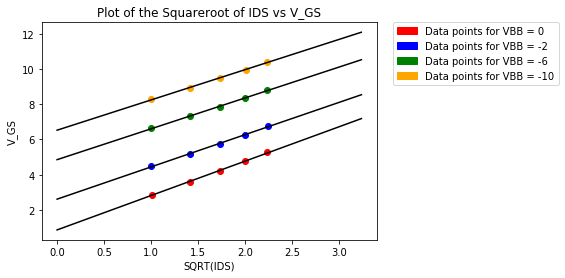
\includegraphics[width=.96\linewidth]{figures/threshold_voltage_plot.png}
    \caption{The plot of $\sqrt{I_{DS}}$ vs $V{GS}$}
    \label{fig:thershold}
\end{figure}
From the graphs we were able to determine the threshold voltage $V_T$ for each $V_{BS}$. 

\begin{table}[ht]
    \begin{tabular}{@{}cc@{}}
    \toprule
    \textbf{$V_{T}$ (V)} & \textbf{$V_{BS}$ (V)} \\ \midrule
    0.867 &         0           \\
    2.61  &        -2           \\
    4.85  &        -6          \\
    6.53  &        -10                   \\
 \bottomrule
\end{tabular}
    \caption{Voltage Threshold at each $V_{BB}$}
    \label{tab:VT}
\end{table}
As we can see the value of $V_t$ when $V_{BB} = 0$ is 0.867V, which is different to the value of $V_T$ that we found in the previous part during the experiment which is 1.58V.From this data we then plotted $V_T$ vs $V_{BS}$, and drew a curve through the points.\\
\begin{figure}[ht]
    \begin{subfigure}[b]{0.40\linewidth}
    \centering
    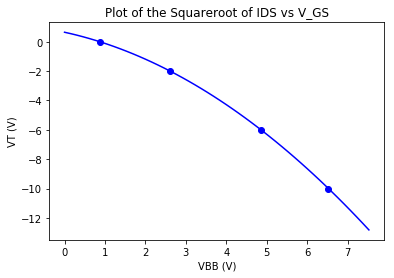
\includegraphics[width=0.95\linewidth]{figures/VT_vs_VBB.png}
    \caption{The plot of $V_t$ vs $V{BS}$}
    \label{fig:thers}
    \end{subfigure}
    \begin{subfigure}[b]{0.40\linewidth}
    \centering
    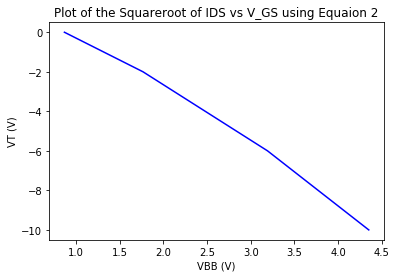
\includegraphics[width=0.95\linewidth]{figures/VT_vs_VBB_EQ2.png}
    \caption{The plot of Equation 2}
    \label{fig:EQ2}
    \end{subfigure}
\end{figure}
From the figure above we can see that the shape of the curve that we plotted with the data we obtained matched that of the shape of the curve that is created with equation 2 in the lab manual. The only difference would depend on the model parameters $\gamma$ and $\phi$.\\
\begin{equation}
    I_{DS} = K(V_{GS} - V_T)^2 
\end{equation}

Is equation 1, from this we know that $\sqrt{K}$ is the slope of the lines in Figure \ref{fig:thershold} we can see that the non-zero values of $V_{BS}$ do not really effect the K parameter. The only thing that is effected is the threshold voltage $V_T$.
\clearpage
\subsection{Semiconductor Parameter Analyzer}

\subsubsection{\texorpdfstring{$I_{DS}$ vs. $V_{DS}$ Characteristics for various $V_{GS}$}{Dump to Source Current vs Voltage Characteristics for various Gate to Source Voltages}}

First we will look at the MOSFET's three terminal characteristics:

\begin{figure}[ht]
    \centering
    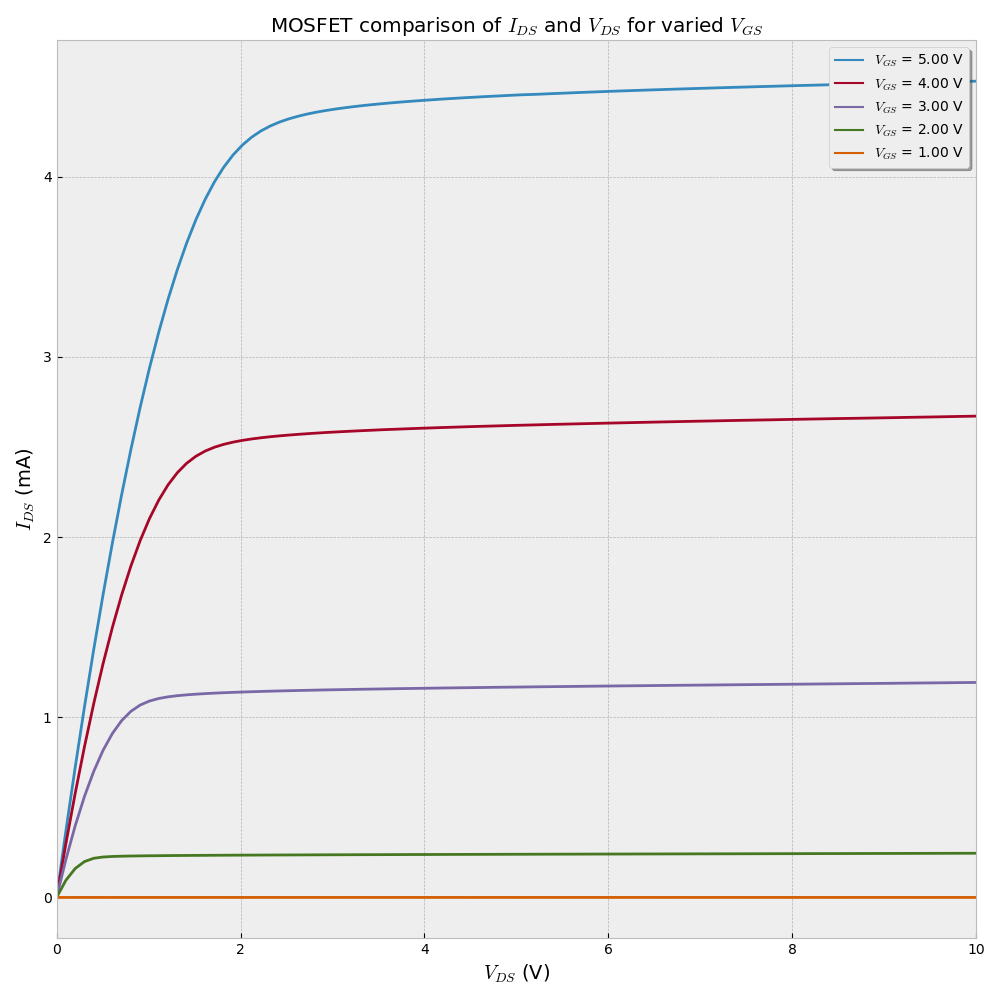
\includegraphics[width=.95\linewidth]{figures/characteristic_nothing.png}
    \caption{The characteristic graphs of $I_{DS}$ vs. $V_{DS}$ for several differing values of $V_{GS}$. }
    \label{fig:characteristic}
\end{figure}

\clearpage

We also view these three terminal characteristics through the Agilent Software, which is shown here:

\begin{figure}[ht]
    \centering
    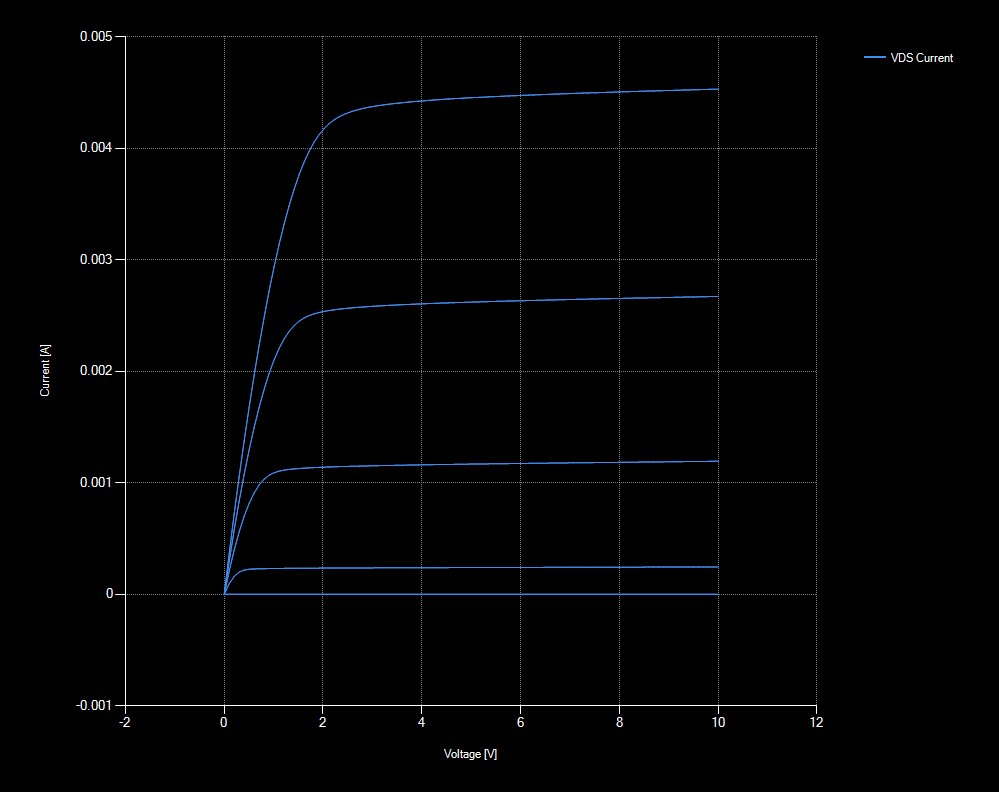
\includegraphics[width=.95\linewidth]{figures/ECE331_Lab3_Data421V1}
    \caption{The characteristic graphs of $I_{DS}$ vs. $V_{DS}$ for several differing values of $V_{GS}$. Shown with in-lab software }
    \label{fig:characteristic_inlab}
\end{figure}

From these graphs we can calculate two important characteristics, these are the MOSFET output resistance $r_o$ and the trans conductance $g_m$.

We note that we can calculate the output resistance by taking two points along a single $V_{GS}$ (The points taken are shown in Figure \ref{fig:VGS_varied}) through $r_o = ( \frac{\partial I_{DS}}{\partial V_{DS}}|_{V_{GS} = constant}$)$^{-1}$. We simply use the delta between the markers where $\Delta V_{DS} \,= \,3.23\; V$  and $\Delta I_{DS} \,= \,75.77\;\mu A$ where $V_{GS}\, = \, 5.00 V$. Therefore $r_o \, = \, 42.63 \;k\Omega$.

We then calculate transconductance $g_m$, where this is defined as $g_m = \frac{\partial I_{DS}}{\partial V_{GS}}|_{V_{DS} = constant}$. The points taken are shown in Figure \ref{fig:VGS_constant}, where the deltas $\Delta V_{GS} \,= \,1.00\; V$  and $\Delta I_{DS} \,= \,1.815\;m A$ where $V_{DS}\, = \, 3.73 V$. Therefore $g_m \, = \, 1.815 \;mS$.

\clearpage

To find the early voltage, the saturation portion of the curves are fitted with a linear function and then the x intercept should be the value of the early voltage. The fitting is completed here, with the fit shown in  Figure \ref{fig:characteristic_tight_fit}. Then the intercepts are found in Figure \ref{fig:characteristic_wide_fit}. We see that there is large variation in the values of early voltage, leading to an experimentally found value of $V_E \, = \, -250 \pm 50 V$.

\begin{figure}[ht]
    \centering
    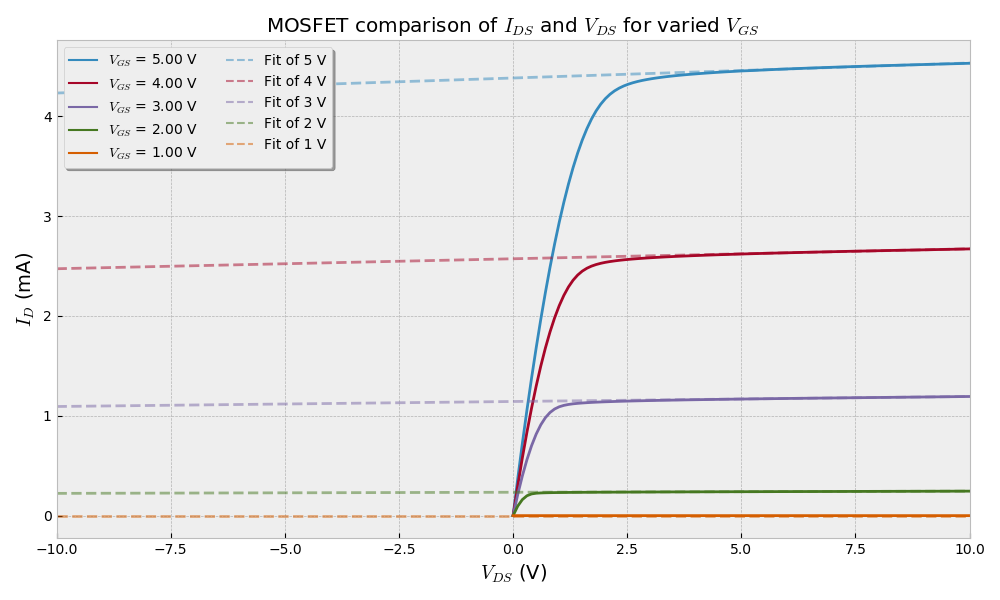
\includegraphics[width=.825\linewidth]{figures/characteristic_tight_fit.png}
    \caption{The characteristic graph with linear fit of saturation portion of curve to show quality of fit.}
    \label{fig:characteristic_tight_fit}
\end{figure}

\begin{figure}[ht]
    \centering
    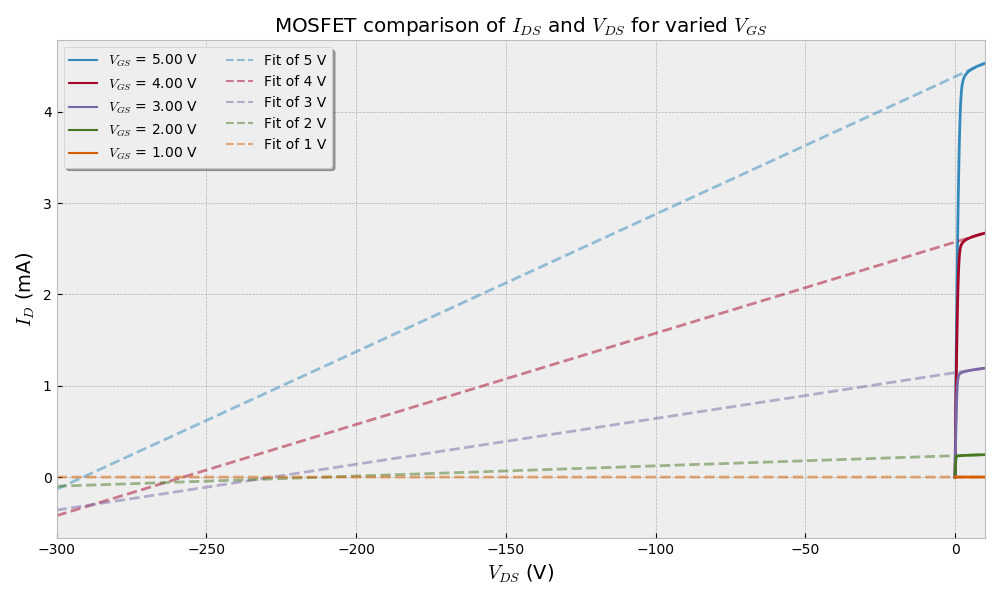
\includegraphics[width=.825\linewidth]{figures/characteristic_wide_fit.png}
    \caption{The characteristic graph with linear fit to show the Early Voltage}
    \label{fig:characteristic_wide_fit}
\end{figure}

\clearpage

To estimate the threshold voltage we graph the value of $I_{DS}$ vs. $V_{GS}$. this is shown in Figure \ref{fig:characteristic_threshold}. Due to the low number of $V_{GS}$ points which are taken, the determination of $V_T$ is a rough approximation. We approximate that it is 1V. This agrees with the found estimated value found during data collection and during part 1, A higher number of $V_{GS}$ points taken would allow for a more accurate approximation.

\begin{figure}[ht]
    \centering
    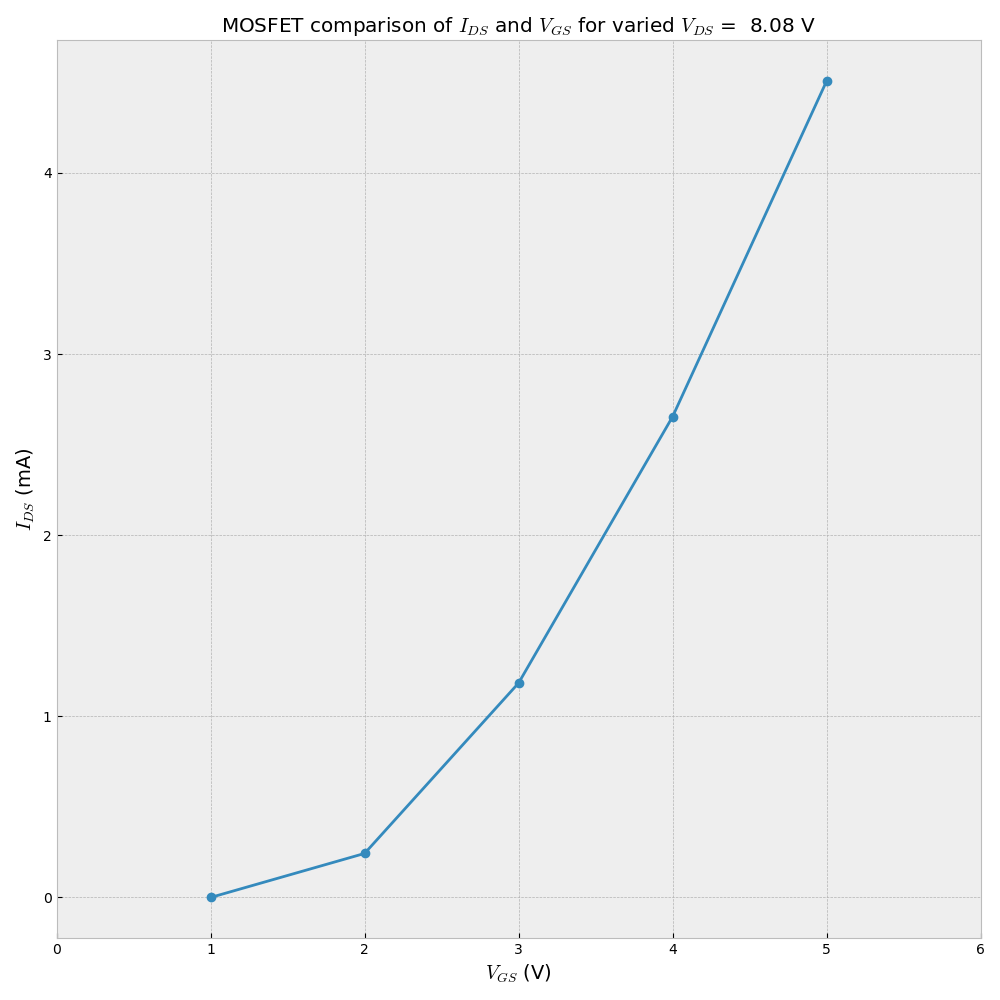
\includegraphics[width=.95\linewidth]{figures/characteristic_threshold.png}
    \caption{The characteristic graph of $I_{DS}$ vs. $V_{GS}$ used for determining the threshold voltage}
    \label{fig:characteristic_threshold}
\end{figure}

\clearpage

Finally for this characteristic graph we show the condition $V_{DS}$ = $V_{GS} - V_T$ which designates the two regions of the graph. These regions correspond to the triode region and the saturation region.

\begin{figure}[ht]
    \centering
    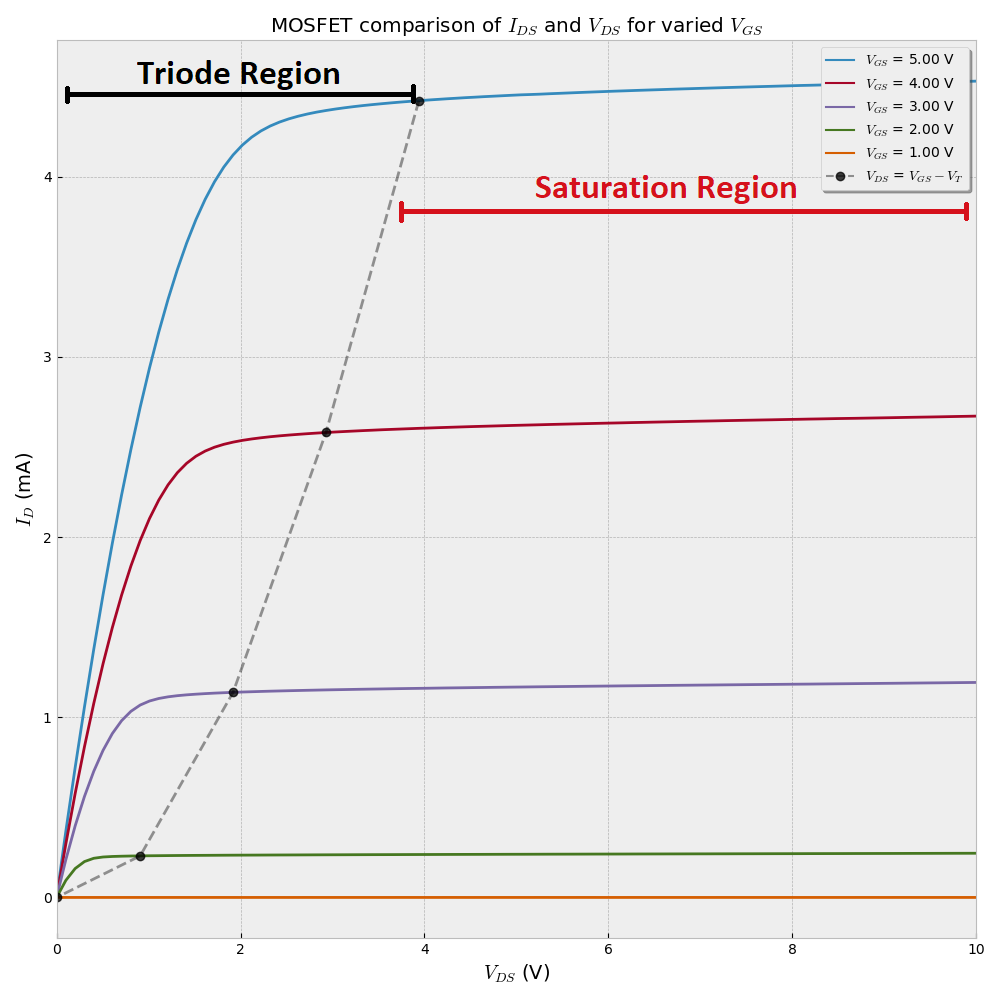
\includegraphics[width=.95\linewidth]{figures/characteristic_intercept_labelled.png}
    \caption{The characteristic graph of $I_{DS}$ vs. $V_{DS}$ with the condition $V_{DS}$ = $V_{GS} - V_T$ inputted and shown on graph}
    \label{fig:characteristic_intercept}
\end{figure}

\clearpage

\subsubsection{\texorpdfstring{$I_{DS}$ vs. $V_{DS}$ Characteristics for various $V_{GS}$ for small $V_{DS}$}{Dump to Source Current vs Small Voltage Characteristics for various Gate to Source Voltages}}

Here we take a look at the characteristic graph of $I_{DS}$ vs. $V_{DS}$ but for small positive and negative values of $V_{DS}$. This is shown in Figure \ref{fig:characteristic_small}. 

We also wish to determine if the MOSFET is behaving as a voltage controlled resistor. We note that a voltage controlled resistor will essentially behave as a passive resistor, except that a third terminal will be able to change the resistance of the device. We note that resistors are linear and in Figure \ref{fig:characteristic_small} we see that the slope of the curve and hence the resistance is controlled by the Gate Voltage. However we also note that the lines are not perfectly linear. These non-linear regions are evidence of distortion in the resistor. We conclude that the MOSFET can be used as a voltage controlled resistor, but care must be taken to avoid distortion effects.

\begin{figure}[ht]
    \centering
    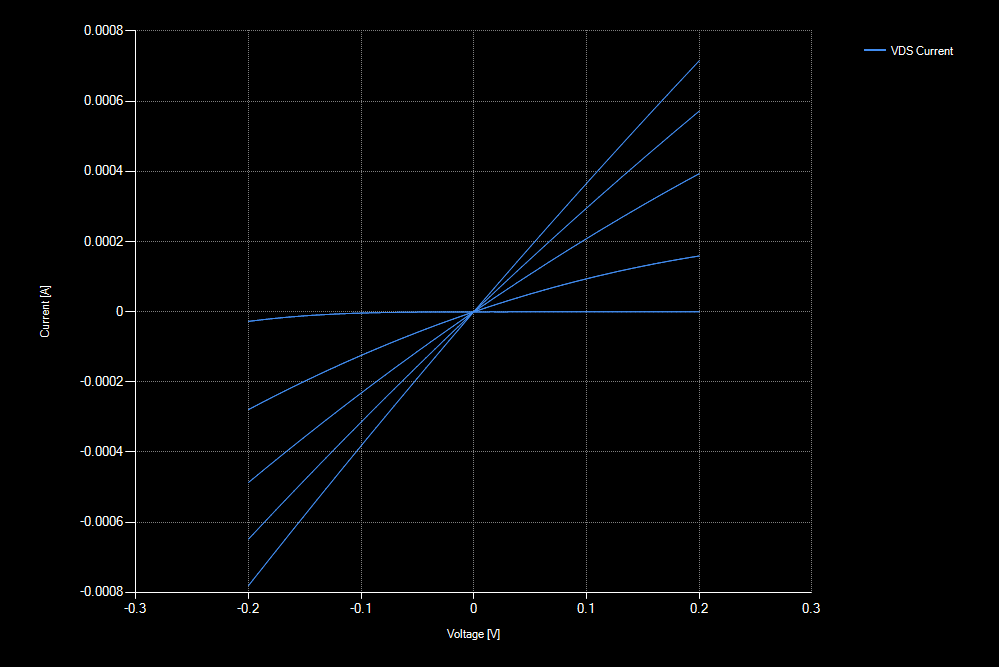
\includegraphics[width=.95\linewidth]{figures/ECE331_Lab3_Data422V1.png}
    \caption{The characteristic graph of $I_{DS}$ vs. $V_{DS}$ with small $V_{DS}$}
    \label{fig:characteristic_small}
\end{figure}
\end{fullreport}

% % % %  PreLab ONLY   % % % %
\begin{prelab}
    \section{Prelab}
    \begin{enumerate}
\item[1.]
\begin{figure}[ht]
    \centering
    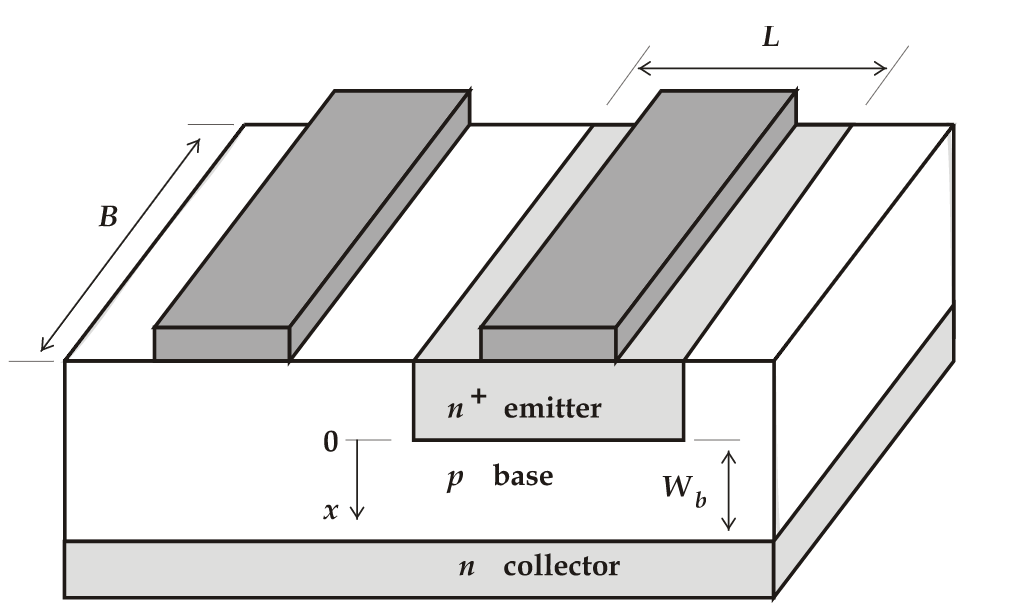
\includegraphics[width=\linewidth]{figures/simple_transistor.PNG}
    \caption{Figure 4 from the lab manual of a simple transistor}
    \label{fig:transitor}
\end{figure}
The figure above is that of a simple transistor from the lab manual. The formula for $I_{CS}$ is:
\begin{equation}
    I_{CS} = \frac{q A_e n_i^2 D_n}{N_{Ab}W_b}
\end{equation}
so if you increase $W_b$ then you are going to lower the gain $\beta_F = \frac{I_C}{I_B}$, but it will increase the switching time


\item[2.]
The three types of materials are:
\begin{labeling}[:]{N\texttt{+} type}
\item [N\texttt{+} type] a n-type semiconductor with a high, often degenerate doping concentration.
\item [N type] a semiconductor that having more conduction electrons than mobile holes.
\item [P type]  a semiconductor having a density of mobile holes in excess of that of conduction electrons.
\end{labeling}


\item[3.]
The four transistor operation modes are:
\begin{labeling}{Reverse-Active}
\item [Saturation] The transistor acts like a short circuit. Current freely flows from collector to emitter.
\item [Cut-off] The transistor acts like an open circuit. No current flows from collector to emitter.
\item [Active] The current from collector to emitter is proportional to the current flowing into the base.
\item [Reverse-Active] Like active mode, the current is proportional to the base current, but it flows in reverse. Current flows from emitter to collector (not, exactly, the purpose transistors were designed for).
\end{labeling}

\item[5.]
The current gain $\beta$ is theoretically constant, but as the question states at high and low values of $I_C$ we see that the the gain decreases. This is due to leakage mechanism in the transistor for low $I_C$ and  due to high level injection for high $I_C$.
\item[6.]
\begin{labeling}{Gummel Plot}
\item [Gummel Plot] A plot which shows $I_C$ versus $V_{BE}$ characteristics of a transistor, this is completed on a semi-log plot where the current is on the log scale.
\item [I\textsubscript{CS}] The collector saturation current is where the base current so that the emitter-base junction is forward biased. In fact, the base current has increased beyond the point where it can cause the collector current flow to increase. At this point, collector emittor currents have increased to a maximal value.
\item [D\textsubscript{n av}] D\textsubscript{n} is the electron diffusion coefficient in the base, which is a physical constant which describing how electrons move through the p-type base. The D\textsubscript{n av} is simply the average of this value throughout the material.
\end{labeling}

\item[7.] The reason that the current gain $\beta \left( \frac{I_C}{I_B} \right) $ decreases at low values of $I_C$ is clear, the ideal model of gain which is shown by $\beta  = \frac{I_C}{I_B}$ is accurate, and hence  $I_C \propto \beta$.

However the reason that the current gain decreases at high values of $I_C$ is not as simple, we deviate from the ideal line equation due to the base resistance and emitter  resistance of the transistor. These resistances are only relevant at high currents as they are non-idealities.

%This is caused because the Voltage ($V_{BE}$) is maintained at a constant value, but when the currents through the device become large the resistances of the emittor and base become significant. This is modelled through the equation: $V_{BE eff} = V_{BE} - \frac{I_{C}}{\beta} r_{bb} - \frac{I_{C}(\beta - 1)}{\beta} r_e$ where $r_e$ and $r_{bb}$ are the emittor and base resistance respectively. There are also other high current effects that come into play


\item[8.]
The differences between the different types of resistors are:
\begin{labeling}{P type pinched resistor}
\item [P type pinched resistor] is a n type region surrounded by a thin p region, known as the pinching region, which is again covered by a n region. It works by lowering the crossectional area and only allowing a small reverse current. These types of resistors can have very high resistances but are often more difficult to manufacture.
\item [P type resistor] is a formed in any one of the isolated regions of p doping, surrounded by a n-region. The differences in resistance are generally controlled by the doping and then crossectional area can also be controlled, but is much larger than the pinched resistors as we only have two layers. 
\item [Carbon resistor] is not a solid state resistor and is not created by using deposition. These different resistance values are generated by varying the length of resistive material that the electricity passes through. This resistive material is made of graphite, ceramic dust and resin.
\end{labeling}

\item[9.]

We see here that the figure below has both the pinched and non-pinched p-type resistor. We know that the calculation of the cross-sectional area will be height times thickness of the resistive material. We note that in our figures, the height will be consistant between both the pinched and unpinched resistor, however the thickness will not be. The thickness of the p-type material will be $t_p$, but the thickness of the pinched resistor will be $t_p - t_n$, since it is deposited above it. This difference in thicness will decrease the area, and effectively increase the resistance.


\begin{figure}[h]
    \begin{subfigure}[b]{\linewidth}
    \centering
    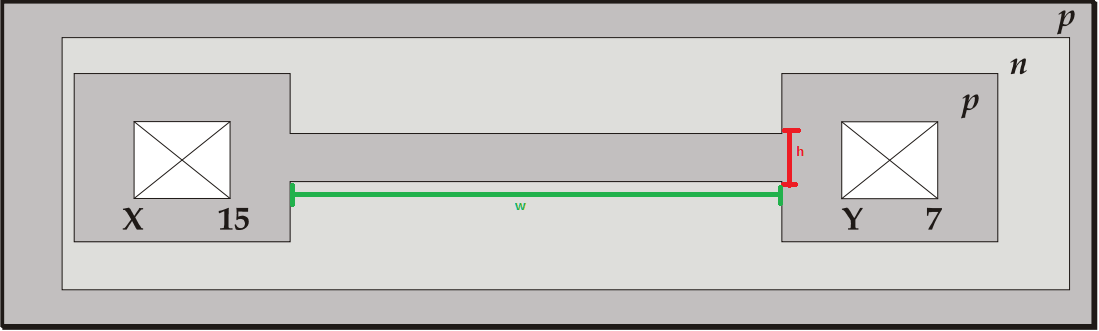
\includegraphics[width=0.95\linewidth]{figures/p_resist.png}
    \caption{Top down diagram of a p-type resistor}
    \label{fig:p_resist}
    \end{subfigure}
    \begin{subfigure}[b]{\linewidth}
    \centering
    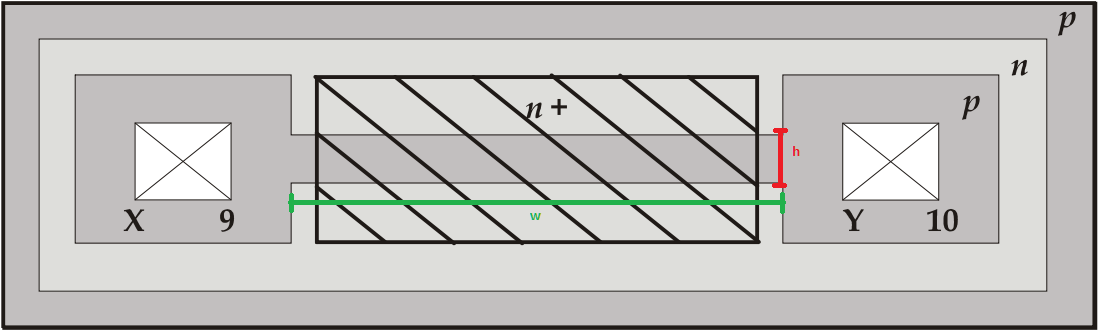
\includegraphics[width=0.95\linewidth]{figures/p_pinched_resist.png}
    \caption{Top down diagram of a p-type pinched resistor}
    \label{fig:pinched_resist}
    \end{subfigure}
\end{figure}

\end{enumerate}

\end{prelab}

% % % %  Data ONLY   % % % %
\begin{data}
    \section{In-Lab Data Collection}
    \subsection{Standard Downward Characteristics}
$R_B = 10.16 \Omega$\\
$R_C = 287.7 \Omega$\\
Here we will study $I_C$ vs $V_{BE}$ characteristics and $\beta$ versus $I_C$ characteristics.

\begin{table}[ht]
    \begin{tabular}{cccc}
\hline
\textbf{$V_{BE}$ (mV)} & \textbf{$I_{B}$ } & \textbf{$V_{CE}$ (V)} & \textbf{$I_{C}$ } \\ \hline
\textit{\textbf{500}} & 0.027 $\mu A$& 1.500  & 0.14 $\mu A$ \\
\textit{\textbf{550}} & 0.088 $\mu A$& 1.500  &0.92  $\mu A$ \\
\textit{\textbf{600}} & 0.280 $\mu A$& 1.499  & 6.02  $\mu A$ \\
\textit{\textbf{650}} & 0.956 $\mu A$&1.500  & 39.76 $\mu A$ \\
\textit{\textbf{700}} & 3.541 $\mu A$ & 1.500  & 259.0 $\mu A$\\
\textit{\textbf{750}} & 0.01295 mA & 1.503  & 1.3666 mA\\
\textit{\textbf{800}} & 0.03919 mA & 1.503  & 4.6170 mA\\
\textit{\textbf{850}} & 0.09654 mA  & 1.523  & 9.1807  mA\\\hline
\end{tabular}
    \caption{Standard Downward Characteristics for transistor 1}
    \label{tab:down}
\end{table}


\subsection{Upwards Operation}

Here we look at the upwards gain of transistor 1 as a function of voltage.

\begin{table}[ht]
    \begin{tabular}{ccccc}
\hline
\textbf{$V_{BE}$ (mV)} & \textbf{$I_{B}$} & \textbf{$V_{CE}$ (V)} & \textbf{$I_{C}$} & $\beta$\\ \hline
\textit{\textbf{550}} & 0.237 $\mu A$ & 1.500  & 1.24  $\mu A$ & 5.232 \\
\textit{\textbf{600}} & 1.465 $\mu A$ & 1.500  & 7.82  $\mu A$ & 5.337 \\
\textit{\textbf{650}} & 9.675 $\mu A$ & 1.501 & 54.82 $\mu A$ & 5.666 \\
\textit{\textbf{700}} & 44.564 $\mu A$ &1.504  & 274.16  $\mu A$ & 6.152\\
\textit{\textbf{750}} & 0.17097 mA & 1.507  & 1.0551 mA  & 6.171\\
\textit{\textbf{800}} & 0.52758 mA & 1.500  & 2.7671 mA & 5.244\\\hline
\end{tabular}
    \caption{Standard Upwards Characteristics for transistor 1}
    \label{tab:up}
\end{table}


\subsection{Base Resistance}

Total Resistance between X and Y in pattern 1 is: $5.021 k \Omega$

Total Resistance between X and Y in pattern 2 is: $61.7 k \Omega$


\subsection{Lateral \textit{pnp} Devices}


We can measure the gain of the lateral pnp transistor by taking the current values of $I_B$ = 0.1007 mA \& $I_C$ = 1.0460 mA at values of $V_CE$ = -1.50 V. This gives a gain of 10.4526. \\

 %\& $V_BE$ = -0.655

We can also measure the gain of the lateral pnp transistor where the outer p diffusion is used as an emitter and the center p diffusion is used as the collector. The value of gain that we get with the currents of $I_B$ = 0.1000 mA\& $I_C$ = 0.0404 mA at values of $V_CE$ = -1.50 V. Giving us a gain of 0.404.

%\& $V_BE$ = -0.691

\end{data}


\end{document}
